
\section{Additional Features}
In order to make the predictions more precise we decided to improve the feature matrix with additional features.
We took into consideration which data could be meaningful for the frequency of bike rentals.
We came to the conclusion that the following 4 features should be added:
\begin{itemize}
\item Age
\item Events
\item Earnings
\item Political Attitude
\end{itemize}
We considered the first point because we assumed that there is a specific age group which uses rental bikes more than others. We conclude from that, if we find stations where a lot of people within this specific age group lives, we will have a higher frequency there. Therefore we investigated in the target group of Santander Rental Bikes and found out that their main target group depicts of people between the age of 16 and 54 \cite{Santander}. Moreover approximately two third of their users are male. That is why we searched for data which gives us the total number of ages as well as the gender for each district in London where Santander provides rental station data. \\\\
Appropriate data was found at the \emph{London Datastore} where data about London's population is freely provided as an excel document \cite{LondonData}. To use this data we first extracted only the district data we are interested in. Since there are ages from 1 to 99 available we created the same age groups like the ones Santander uses for their survey data and summed up the according values. Since we know that males using bikes more often we assigned the age group data to females as well as to males seperately. With this task the data cleansing part was done. How the data was prepared further will be explained in the following chapter \ref{sec:dpadditional} Data Preparation.\\\\
Another feature we wanted to take into account is event data. We assume that when more events take place at a specific location, more people will visit this location and out of that more stations around this corresponding location will be used.
For this purpose we instructed Ankur Mehra, who has done web scraping tasks before, to scrape appropriate data. The tasks was to find a source which provides event data of London over the last 4 years.\\\\
Event data was scraped from \emph{LondonTown.com}\cite{LondonTown2019}. The description of the implementation can be found in the report of Ankur Mehra.\\\\
Santander distinguishes between \emph{Casual Users} which use their bikes occasionally and just pay per ride and \emph{Members} which have their own keys and pay beforehand to use bikes for one year. According to their last user survey they own more members than casual users. Moreover they found out that members have a higher average annual income than casual users, we investigated in income data as well. Our assumption was the districts in which more people with a higher income live are the districts where more potential members live and therefore where more frequency will take place.\\\\
The \emph{Office for National Statistics} provides data of earnings in the UK from 2018, which we used as a source~\cite{OfficeforNationalStatistics2019}. The data cleansing part consisted of extracting the data of the 15 districts we are interested in which can be seen in figure~\ref{fig:earnings}.
\begin{figure}[H]
\centering
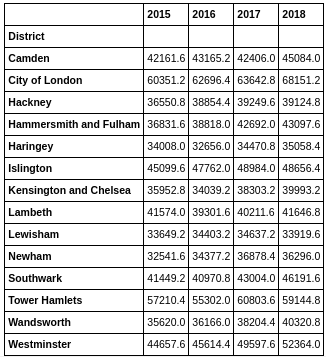
\includegraphics[width=0.6\textwidth]{img/earnings}\label{fig:earnings}
\captionof{figure}{Cleaned earnings data}\label{fig:earnings}
\end{figure}
The last additional feature we took into account was the political attitude. Since using bikes instead of cars or public transportation is healthier and more environmental friendly, we assume that the most Santander users are interested in health, environmental protection and climate protection. Therefore we investigated in which parties have the most content according to those subjects, because we assume that voter of those parties will be more likely to use Santander bikes. Therefore districts with the most voters of according parties will show a higher frequency of rental bike usage.\\\\
Therefore we researched for specific content of election programs of the several parties within the UK.
We found out that that the \emph{UK Independence Party} have mentioned least content regarding health and climate. Slightly more information was found in the election program of the \emph{Liberal Democrats} as well as the \emph{Conservatives}. The most content to health, climate and environment was found on the agenda of the \emph{Labour Party} as well as the \emph{Green Party} \cite{SandraLavilleJohnSauven2017}.\\ Therefore we assumed that districts with a high amount of Labour Party and Green Party voters will use rental bikes more often than other districts.\\\\
We searched for according data and were resourceful once again at the London Datastore. Here we found Data of the last four elections. We used the data of the election from 2016 and once again extracted all the data from the districts we are interested in.\\
Nevertheless those are all just assumptions. Of course there are several other reasons than trying to live healthier or doing something good for the environment, to use rental bikes. A lot of people will use it probably only because it is fun, cheaper and they may not have a driving license for cars.
\subsection{Data Preparation}\label{sec:dpadditional}
\subsubsection{District to Stations}

Nearly all of the additional data is stored by London district.
To be used with our stations, we need to assign to every station a corresponding
district.
We first determined the centroid of the districts using Nominatim, which we compared
to each station's coordinates to keep the closest district to each station.
This enables us to link the \emph{age}, \emph{earnings} and \emph{political attitude}
datasets the stations.

\subsubsection{Filling Missing Years}

The data we extracted doesn't necessarily contain data for the same duration as our
bike rental data. Thankfully, some data don't check much during a few years like
\emph{age}, \emph{earnings} and possibly \emph{political attitude} as well.
With this supposition, we decided to fill missing periods with the closest data
we have.

\subsubsection{Events}

First, the events are located with a postcode and a street, so we use Nominatim to extract
their coordinates. For a few postcodes, we have to use Geonames as some are missing
or no more used officially. Last, there is an event called ``secret cinema'' which
happens at a location that is disclosed shortly before the rendez-vous time, so
the postcode and street given don't exist.

Second, the date field follows many different formats, from a single date, to a list,
or a range. Here is a list of different formats found:
\begin{itemize}
    \item day month year
    \item day-of-week day month year
    \item day --- day month year
    \item day-of-week day --- day-of-week day month year
    \item day month --- day month year
    \item day month to day month year
    \item day and day month year
    \item day, day and day month year
    \item day month, day month and day month year
    \item 15th May --- 05th March 2016
    \item Various Venues
    \item \ldots{}
\end{itemize}

We had to implement different RegEx parsing in order to parse all possibilities
found in the database.
Once parsed, we transformed the dates into a list of date
(so ``15th May --- 15th June 2019'' creates 32 days between those two dates included)
to store each event each day it appears.

Finally, we created two features for each day in our original features dataset.
For each day, we take the distance to the closest event and we count the number
of events in a close perimeter (3 kilo-meters for instance).

\subsection{Data Evaluation}

\subsubsection{Demographic, Earnings, Political Attitude}
The demographic, earnings and political attitude data per district has been
placed in a table shown in figure~\ref{fig:addition_features}.
\begin{figure}[H]
\centering
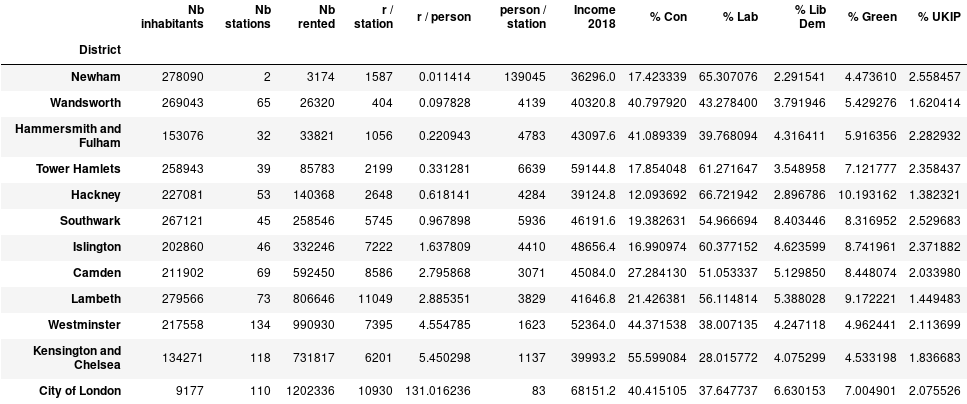
\includegraphics[width=\textwidth]{img/additional_features}\label{fig:addition_features}
\captionof{figure}{Additional data per district}\label{fig:addition_features}
\end{figure}

We can see that the district with the most rented bikes has also nearly the most
station, but has the least amount of person living in it. This is the \emph{City
of London}.
The City is a district used mostly as a workplace by Londoners and many of them
live in other districts, so this might suggest that people are more likely to
rent a bike near their workplace than near their living place.
It might then be more useful to obtain the data based on where people work
(and possibly also where they go shopping and have a meal) rather than where
people live, but this kind of information isn't usually available.

Furthermore, since it was decided to use a different learning model for each station,
the \emph{age}, \emph{earnings} and \emph{political attitude} datasets might not add
much accuracy. They could, however, be used to predict the usage of a new station
based on its location to determine whether it is relevant to proceed with construction
or not.

\subsubsection{Events}

Concerning the events additional feature, it might be interesting to have more
accurate information about the events: hour, duration, amount of people expected,
kind of place/kind of event, \ldots{}
Indeed, if the event takes place too late in the evening or involves drinking
alcohol (if it is in a bar for example), people might not be wanting to use a bike.
Also, if it doesn't expect many people to come, there won't be any noticeable change
in the amount of bike rented.
Additionally, some events last for nearly a year and might not create bike rental
change during this whole period, rather at some precise dates but we don't have
any details.
